\documentclass[12pt]{article}

% Configuración básica
\usepackage[spanish]{babel}
\usepackage[utf8]{inputenc}
\usepackage[T1]{fontenc}
\usepackage{geometry}
\usepackage{setspace}
\usepackage{hyperref}
\usepackage{enumitem}
\usepackage{graphicx}
\usepackage[section]{placeins}
\usepackage{float}

\geometry{letterpaper, margin=2.5cm}
\onehalfspacing

% Datos del informe (puedes modificarlos)
\title{Evidencia 9 \\ Reporte de Depuración y Evaluación de Componentes de Software}
\author{David Armando Ramírez Navarrete}
\date{30 de marzo de 2026}

\begin{document}

\maketitle

\section*{Resumen}
El presente informe técnico documenta la ejecución de pruebas funcionales y técnicas realizadas durante el desarrollo de las prácticas profesionales, con el objetivo de validar el comportamiento esperado de funcionalidades asociadas a un cambio controlado. La actividad incluyó la revisión de criterios de aceptación, la ejecución de casos de prueba, el registro de resultados obtenidos, la integración de evidencias visuales y la validación técnica mediante checklist y soportes documentales.

Las pruebas se desarrollaron en un entorno controlado y con acceso restringido, a fin de proteger la confidencialidad de la información y evitar la exposición de sistemas o datos sensibles. Como resultado, se obtuvo una cobertura total de los casos de prueba ejecutados, con avance del 100\% y resultados satisfactorios en los escenarios evaluados. Asimismo, se verificó la mitigación del riesgo mediante el indicador RMP y se documentó la validación técnica correspondiente.

El trabajo evidencia competencias en análisis funcional, ejecución de pruebas, validación técnica, interpretación de resultados y documentación estructurada de evidencias, alineadas con el perfil profesional de Ingeniería en Sistemas.

\section*{Introducción}

La ejecución de pruebas y la validación de funcionalidades constituyen actividades esenciales para asegurar la calidad de los cambios implementados en un entorno técnico-profesional. A través de estas actividades es posible comprobar que los desarrollos o ajustes realizados cumplan con los criterios de aceptación definidos, operen correctamente en los escenarios previstos y no generen afectaciones en procesos existentes.

En el contexto de las prácticas profesionales, se participó en la ejecución de pruebas asociadas a una funcionalidad específica, integrando tanto validaciones funcionales como revisiones técnicas. Para ello, se utilizaron instrumentos de apoyo previamente elaborados, tales como estrategia y plan de pruebas, checklist de validación, reportes de ejecución, evidencias visuales y soporte documental técnico. Esta base permitió dar continuidad al trabajo realizado previamente en materia de documentación técnica y control de calidad.

El presente informe tiene como propósito documentar la ejecución de estas pruebas, describiendo el proceso seguido, los resultados obtenidos, los hallazgos identificados y la forma en que se validó el cumplimiento funcional y técnico del cambio evaluado.

\section*{Objetivo general}

Validar el funcionamiento funcional y técnico de una funcionalidad implementada mediante la ejecución estructurada de pruebas, el registro de evidencias y la verificación del cumplimiento de criterios de aceptación y validación técnica.

\section*{Alcance}

La presente evidencia se limita a la documentación del proceso de ejecución de pruebas y validación de una funcionalidad específica en un entorno controlado. El informe incluye la revisión de criterios de aceptación, la ejecución de casos de prueba, el análisis de resultados, la integración de evidencias visuales, la verificación técnica y el soporte documental correspondiente.

Por razones de confidencialidad, no se incluyen nombres completos de sistemas internos, usuarios reales, credenciales, rutas sensibles ni información propietaria de la organización. La información se presenta de manera general y académicamente estructurada.

\section*{Descripción de la actividad realizada}

La actividad desarrollada consistió en la ejecución de pruebas funcionales y técnicas sobre una interfaz de usuario correspondiente a un cambio controlado. La validación se realizó a partir de casos de prueba previamente definidos, criterios de aceptación establecidos y soportes documentales asociados al proceso de revisión técnica.

En la parte funcional, se ejecutaron escenarios orientados a verificar que el usuario pudiera acceder a la funcionalidad, visualizar información esperada y completar acciones específicas conforme a las reglas del negocio. Los resultados se documentaron mediante capturas de pantalla, tablas de resultados esperados contra resultados obtenidos y reportes de cobertura de ejecución.

En la parte técnica, se revisó la validación del cambio mediante checklist especializado, verificación en entorno controlado y revisión de soportes documentales obligatorios, asegurando que el componente evaluado cumpliera con los requisitos necesarios para considerarse validado.

\section*{Metodología de ejecución}

La metodología aplicada para la ejecución de pruebas se desarrolló en las siguientes etapas:

\begin{enumerate}[label=\arabic*.]
    \item \textbf{Revisión de documentación de prueba.} Se consultaron los instrumentos de apoyo previamente definidos, incluyendo estrategia y plan de pruebas, criterios de aceptación, checklist de validación y formatos de evidencia. Esto permitió contar con una base clara para la ejecución.

    \item \textbf{Identificación de criterios de aceptación.} Se revisaron los criterios funcionales esperados para la historia o cambio evaluado. En las evidencias proporcionadas se observa, por ejemplo, que uno de los criterios establece que determinadas transacciones fueron desarrolladas y certificadas de manera exitosa, lo cual sirvió como referencia para la validación del comportamiento esperado.

    \item \textbf{Ejecución de casos de prueba.} Se ejecutaron los casos de prueba definidos sobre la funcionalidad evaluada, registrando para cada uno la condición y datos de entrada, la descripción del caso, el resultado esperado, el resultado obtenido y el estatus final.

    \item \textbf{Registro de evidencias funcionales.} Cada caso ejecutado fue respaldado con evidencia visual, documentando pantallas, navegación y resultados observados durante la prueba.

    \item \textbf{Validación técnica.} De forma complementaria, se realizó la revisión técnica del cambio mediante checklist y verificación documental, integrando evidencia de ejecución en un entorno controlado y soporte relacionado con el cambio.

    \item \textbf{Consolidación de resultados.} Finalmente, los resultados se concentraron en un reporte general de ejecución que permitió medir cobertura, avance, estatus y mitigación del riesgo.
\end{enumerate}

\section*{Resultados obtenidos}

Los resultados observados muestran una ejecución satisfactoria y bien documentada. En el reporte general de ejecución se aprecia que se ejecutaron tres casos de prueba, todos con estatus satisfactorio, lo que representa un avance de ejecución del 100\%. Asimismo, no se reportan casos insatisfactorios, bloqueados, cancelados ni erróneos. Esto permite afirmar que la funcionalidad evaluada respondió correctamente en los escenarios probados.

Adicionalmente, se observa un indicador RMP (Riesgo Mitigado por Pruebas) de 100, asociado a una clasificación de riesgo bajo. Este valor sugiere que la cobertura ejecutada, la complejidad funcional atendida y la remoción de defectos permitieron una validación completa del cambio dentro del alcance de la prueba.

En las tablas de ejecución por caso de prueba también se aprecia que los resultados obtenidos fueron registrados como satisfactorios, en concordancia con los resultados esperados definidos previamente. Esto fortalece la trazabilidad entre lo planeado y lo ejecutado.

\section*{Análisis de evidencias presentadas}

\textbf{Figura 1. Reporte general de ejecución.} La captura del reporte general muestra el consolidado de la ejecución de casos de prueba. Se identifican tres casos ejecutados, todos satisfactorios, con cobertura total del 100\%. También se observa el cálculo del RMP, cuyo valor de 100 refleja un nivel adecuado de mitigación del riesgo mediante pruebas.

\textbf{Figura 2. Evidencia visual del caso CP1.} En la hoja de evidencias se documenta el caso CP1, cuyo resultado esperado indica que el usuario debe poder visualizar portafolios y guardar alguno de ellos. Las capturas de pantalla permiten observar el flujo funcional ejecutado y respaldan que la navegación y visualización ocurrieron conforme a lo esperado.

\textbf{Figura 3. Registro de resultados esperados y obtenidos.} La tabla del caso de prueba muestra la relación entre condición de entrada, pasos ejecutados, resultado esperado y resultado obtenido. En los casos visibles, el resultado fue clasificado como satisfactorio, lo que demuestra consistencia entre el comportamiento esperado y el observado.

\textbf{Figura 4. Evidencia de verificación técnica.} Las capturas del PDF de evidencia muestran la revisión y verificación en entorno controlado. En una de ellas se observa el mensaje de verificación exitosa y ausencia de error, lo que sirve como respaldo técnico del cambio evaluado.

\textbf{Figura 5. Checklist de validación técnica.} La imagen del checklist técnico muestra responsables, verificadores, observaciones y soportes documentales vinculados al proceso de validación. Esta evidencia es importante porque demuestra que la prueba no se limitó al comportamiento funcional, sino que también incluyó control documental y validación técnica formal.

\section*{Hallazgos}

Con base en la información visible en las evidencias, no se identifican incidencias funcionales críticas dentro de los casos ejecutados, ya que todos fueron clasificados como satisfactorios y el reporte general no muestra defectos activos derivados de esta ejecución.

Sin embargo, desde una perspectiva técnica y documental, sí se observa que parte del proceso de validación incluye observaciones relacionadas con soporte documental y control de versiones del documento. Esto permite señalar como hallazgo metodológico que la validación integral de un cambio no solo depende del comportamiento funcional, sino también de la correcta integración de evidencias, documentos y revisiones técnicas.

\section*{Beneficios de la actividad}

La ejecución de pruebas y la validación de funcionalidades generaron beneficios relevantes tanto a nivel técnico como formativo:

\begin{itemize}
    \item permitió comprobar el comportamiento esperado de la funcionalidad evaluada;
    \item fortaleció la trazabilidad entre criterios de aceptación, ejecución y evidencia;
    \item confirmó la cobertura total de los escenarios definidos dentro del alcance;
    \item contribuyó a la mitigación del riesgo asociado al cambio mediante pruebas;
    \item reforzó el uso de documentación técnica y checklist como apoyo al control de calidad;
    \item favoreció el desarrollo de habilidades de análisis, validación y documentación técnica.
\end{itemize}

\section*{Conclusiones}

La actividad desarrollada permitió validar de manera satisfactoria una funcionalidad implementada mediante la ejecución estructurada de pruebas funcionales y técnicas, respaldadas con evidencia visual, reporte general de ejecución y checklist de validación. Los resultados obtenidos muestran que los casos de prueba ejecutados cumplieron con los criterios esperados y alcanzaron una cobertura total del 100\%, sin registrar casos fallidos dentro del alcance evaluado.

Asimismo, el uso complementario de instrumentos como el reporte de ejecución, el indicador RMP, las evidencias de caso y la validación técnica documental permitió realizar una revisión más completa del cambio, integrando no sólo la verificación funcional, sino también el control técnico y documental asociado.

En términos formativos, esta actividad fortaleció competencias relacionadas con ejecución de pruebas, análisis de resultados, control de calidad, validación técnica y documentación estructurada, contribuyendo al perfil profesional de Ingeniería en Sistemas y a la comprensión integral del proceso de aseguramiento de calidad en entornos profesionales.

\section*{Referencias}

\begin{itemize}
    
    \item Agile Alliance. (n.d.). \textit{Agile Basics}.  
    Recuperado de: \url{https://agilealliance.org/agile101/agile-basics/}

    \item Atlassian. (n.d.). \textit{¿Qué es Scrum?}.  
    Recuperado de: \url{https://www.atlassian.com/es/agile/scrum}
    
    \item DataCamp. (n.d.). \textit{Python try-except: Exception handling explained}.  
    Recuperado de: \url{https://www.datacamp.com/tutorial/python-try-except}

    \item DataCamp. (n.d.). \textit{Python f-strings: Everything you need to know}.  
    Recuperado de: \url{https://www.datacamp.com/tutorial/python-f-string}

    \item DocuMind. (n.d.). \textit{Technical writing best practices}.  
    Recuperado de: \url{https://www.documind.chat/blog/technical-writing-best-practices}

    \item Google. (n.d.). \textit{Importar y exportar archivos}.  
    Recuperado de: \url{https://support.google.com/docs/answer/3093340?hl=es-419}

    \item Google. (n.d.). \textit{Convertir archivos a Google Docs}.  
    Recuperado de: \url{https://support.google.com/docs/answer/3093197?hl=es-419}

    \item Google Cloud. (n.d.). \textit{Cómo crear campos calculados en Looker Studio}.  
    Recuperado de: \url{https://docs.cloud.google.com/looker/docs/studio/tutorial-create-calculated-fields-in-looker-studio?hl=es-419}

    \item Google Cloud. (n.d.). \textit{Variables de resultado de consulta en Looker Studio}.  
    Recuperado de: \url{https://docs.cloud.google.com/looker/docs/studio/query-result-variables?hl=es-419}

    \item Google Cloud. (n.d.). \textit{Agregar, editar y solucionar problemas con campos calculados en Looker Studio}.  
    Recuperado de: \url{https://docs.cloud.google.com/looker/docs/studio/add-edit-and-troubleshoot-calculated-fields?hl=es-419}

    \item Google Workspace Developers. (n.d.). \textit{Google Apps Script overview}.  
    Recuperado de: \url{https://developers.google.com/apps-script/overview}

    \item Google Workspace Developers. (n.d.). \textit{Best practices for Google Apps Script}.  
    Recuperado de: \url{https://developers.google.com/apps-script/guides/support/best-practices}

    \item Google Workspace Developers. (n.d.). \textit{Custom menus in Google Sheets}.  
    Recuperado de: \url{https://developers.google.com/apps-script/guides/menus}

    \item Google Workspace Developers. (n.d.). \textit{Spreadsheet service}.  
    Recuperado de: \url{https://developers.google.com/apps-script/reference/spreadsheet}

    \item Google Workspace Developers. (n.d.). \textit{Calendar service}.  
    Recuperado de: \url{https://developers.google.com/apps-script/reference/calendar}

    \item Google Workspace Developers. (n.d.). \textit{Tasks API overview}.  
    Recuperado de: \url{https://developers.google.com/tasks}

    \item InvGate. (n.d.). \textit{Documentación técnica: mejores prácticas, formatos y ejemplos}.  
    Recuperado de: \url{https://blog.invgate.com/es/documentacion-tecnica}

    \item ISO. (n.d.). \textit{ISO 9001 — Documented information}.  
    Recuperado de: \url{https://www.iso.org/standard/62085.html}

    \item Python Software Foundation. (n.d.). \textit{Built-in exceptions}.  
    Recuperado de: \url{https://docs.python.org/3/library/exceptions.html}

    \item Python Software Foundation. (n.d.). \textit{PEP 8 -- Style Guide for Python Code}.  
    Recuperado de: \url{https://peps.python.org/pep-0008/}

    \item Real Python. (n.d.). \textit{Python Exceptions: An Introduction}.  
    Recuperado de: \url{https://realpython.com/python-exceptions/}

    \item Schwaber, K., \& Sutherland, J. (2020). \textit{La Guía Scrum}.  
    Recuperado de: \url{https://scrumguides.org/docs/scrumguide/v2020/2020-Scrum-Guide-Spanish-Latin-South-American.pdf}

    \item Scrum Guides. (n.d.). \textit{Scrum Guide – Downloads}.  
    Recuperado de: \url{https://scrumguides.org/download.html}

\end{itemize}

\appendix
\section{Evidencias gráficas de la Actividad 9}

\begin{figure}[H]
    \centering
    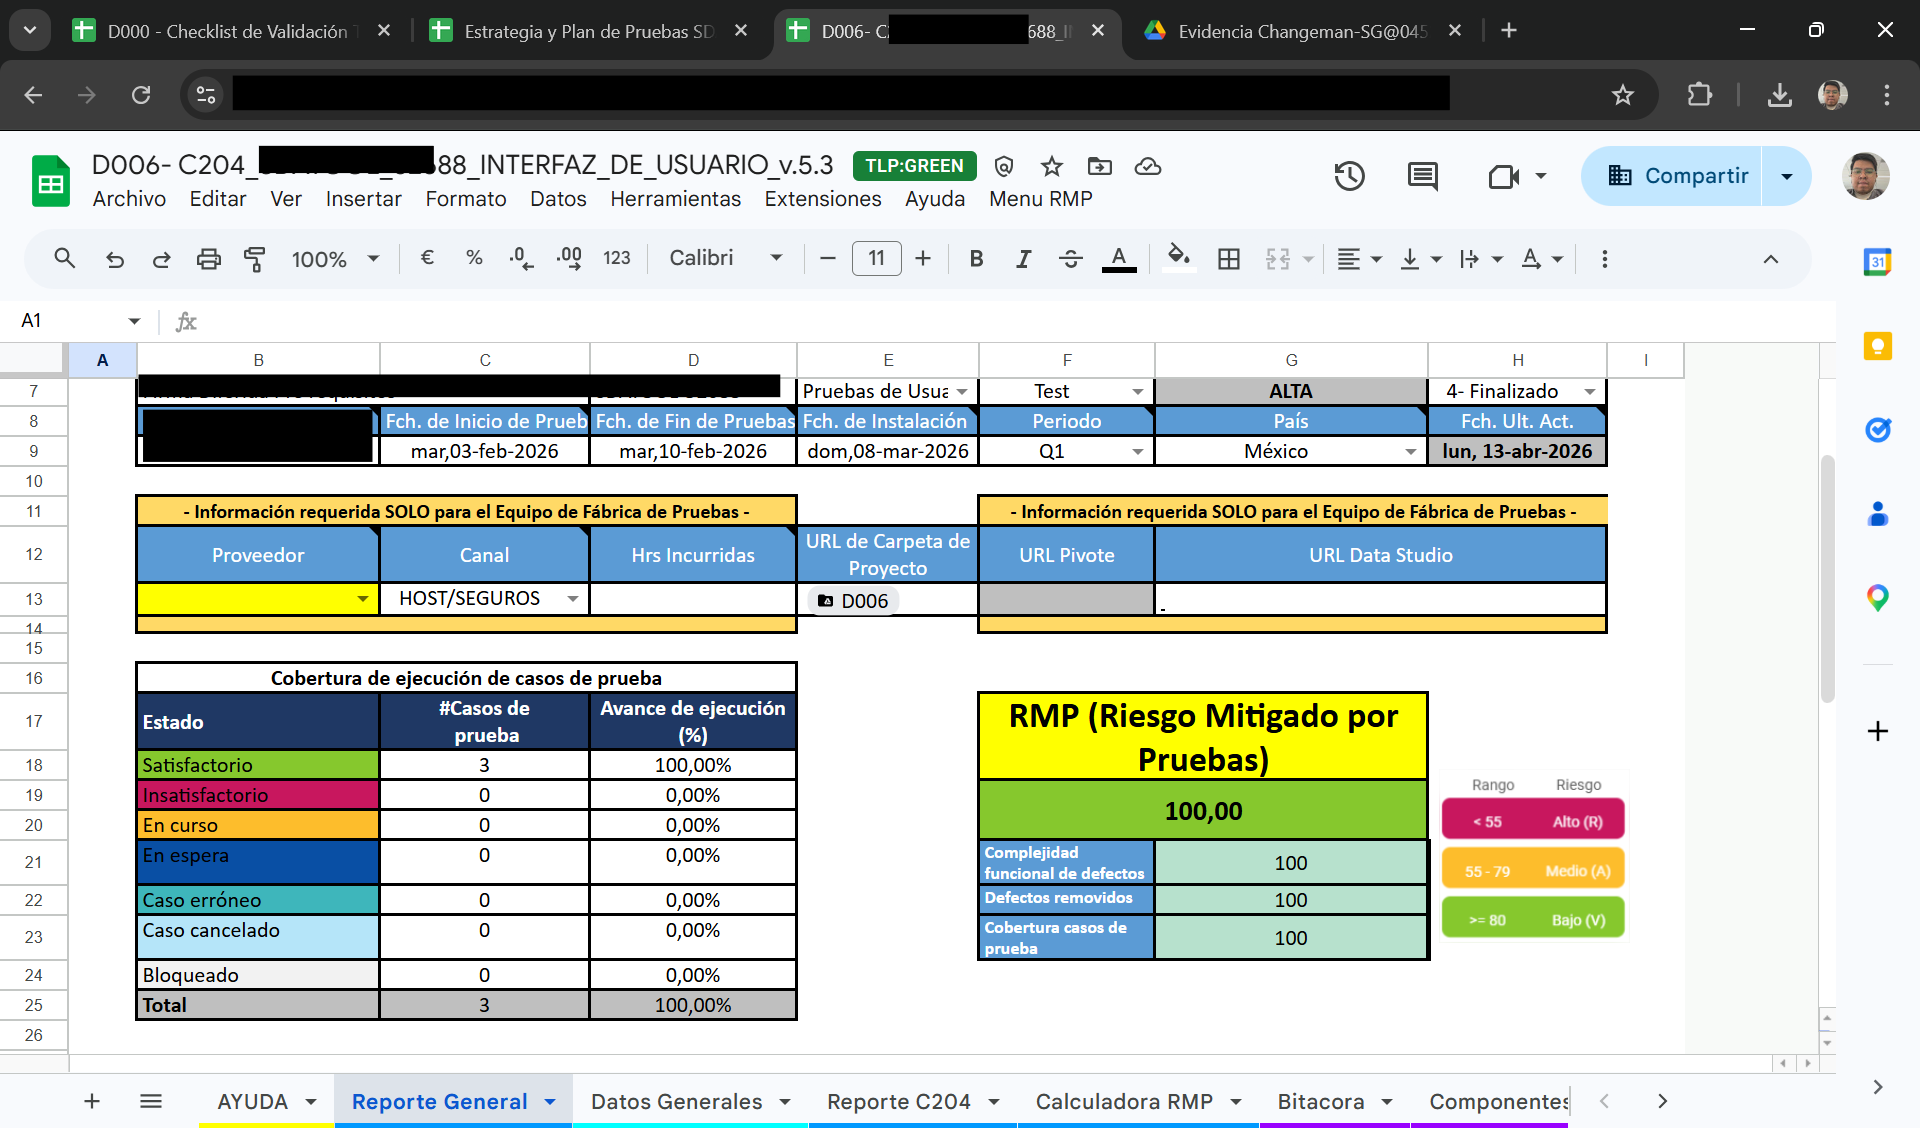
\includegraphics[width=0.95\textwidth]{E9/E1.png}
    \caption{Reporte general de ejecución de casos de prueba, donde se observa la cobertura total, el avance del 100\% y el indicador RMP con riesgo mitigado por pruebas.}
\end{figure}

\begin{figure}[H]
    \centering
    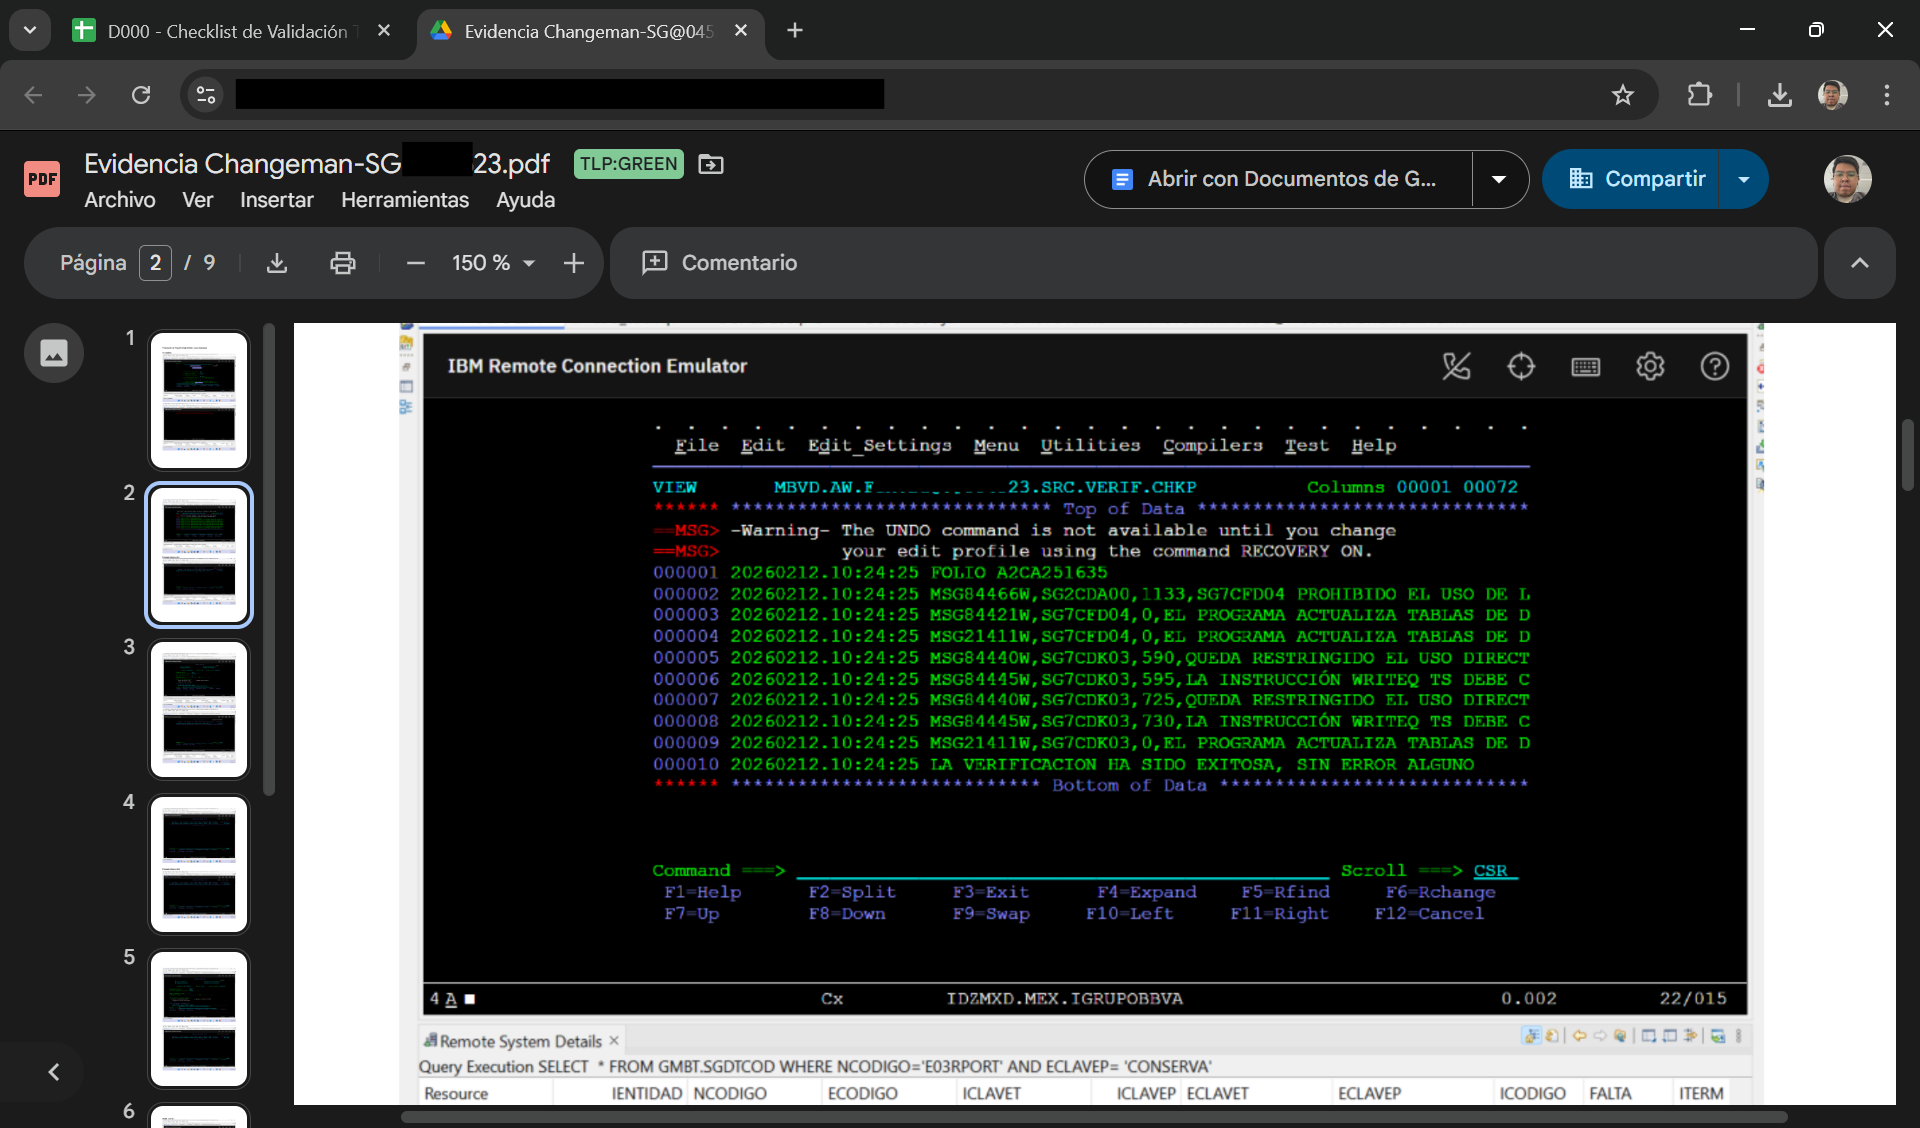
\includegraphics[width=0.95\textwidth]{E9/E2.png}
    \caption{Evidencia funcional del caso de prueba CP1, en la que se documenta visualmente la navegación y el comportamiento esperado de la funcionalidad evaluada.}
\end{figure}

\begin{figure}[H]
    \centering
    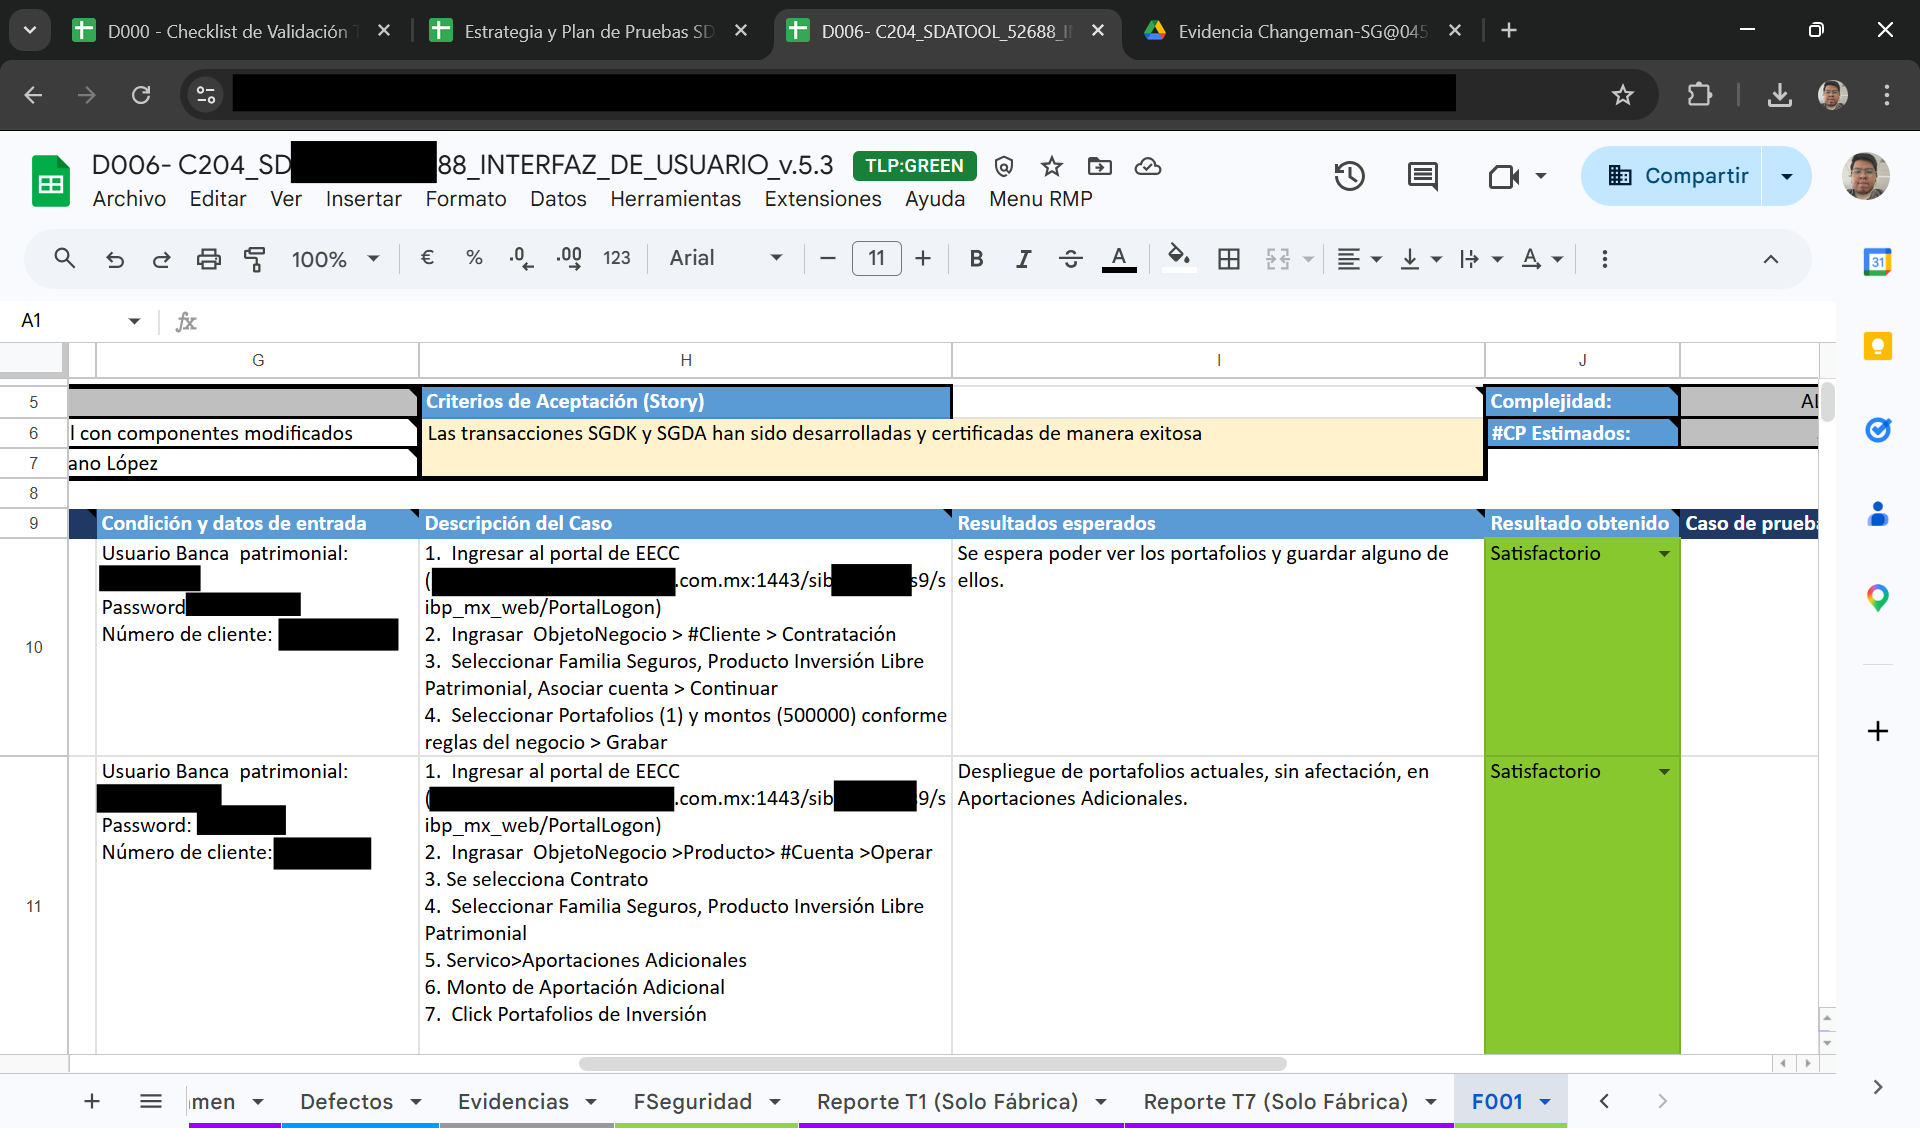
\includegraphics[width=0.95\textwidth]{E9/E3.png}
    \caption{Registro de casos de prueba con condición de entrada, descripción del caso, resultados esperados y resultado obtenido, mostrando estatus satisfactorio en los escenarios ejecutados.}
\end{figure}

\begin{figure}[H]
    \centering
    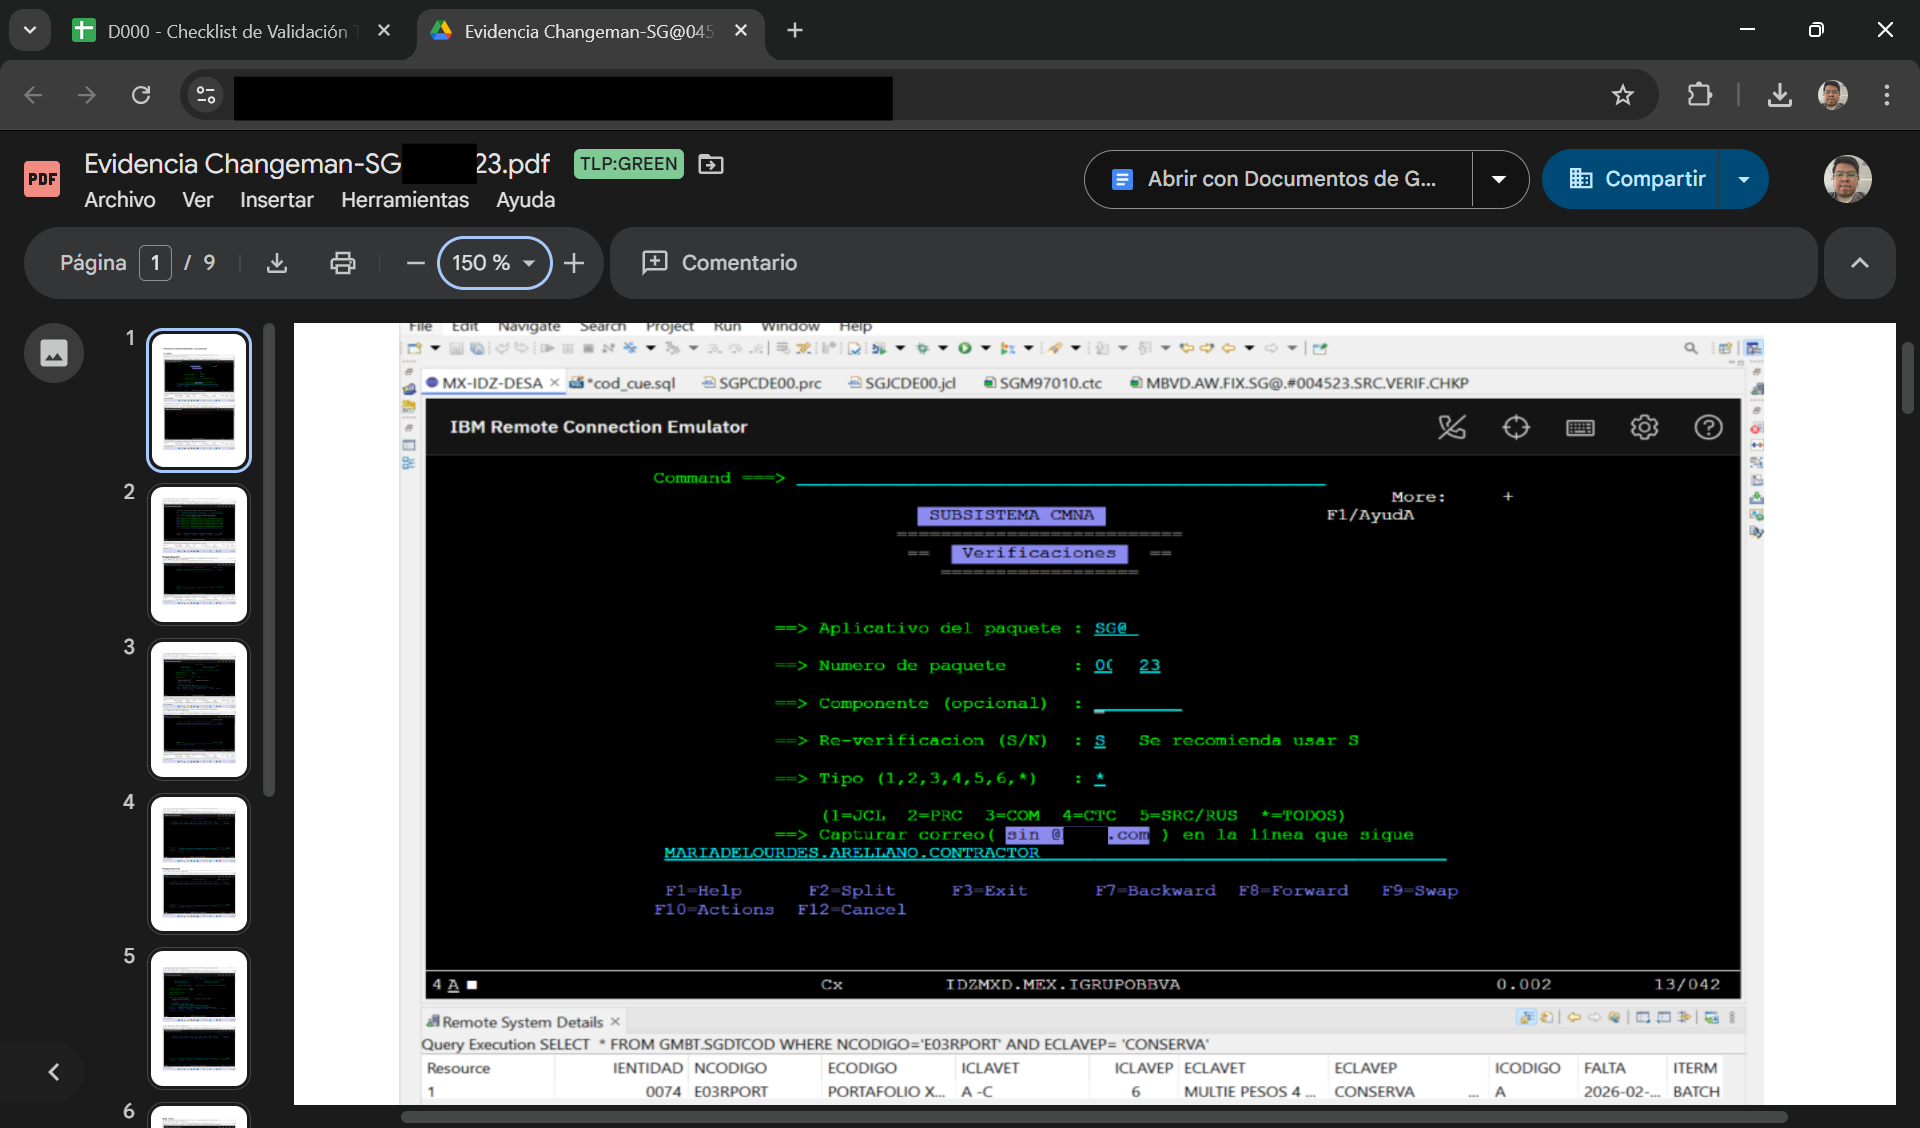
\includegraphics[width=0.95\textwidth]{E9/E4.png}
    \caption{Evidencia de verificación técnica del cambio en entorno controlado, utilizada como soporte de validación complementaria al proceso de pruebas funcionales.}
\end{figure}

\begin{figure}[H]
    \centering
    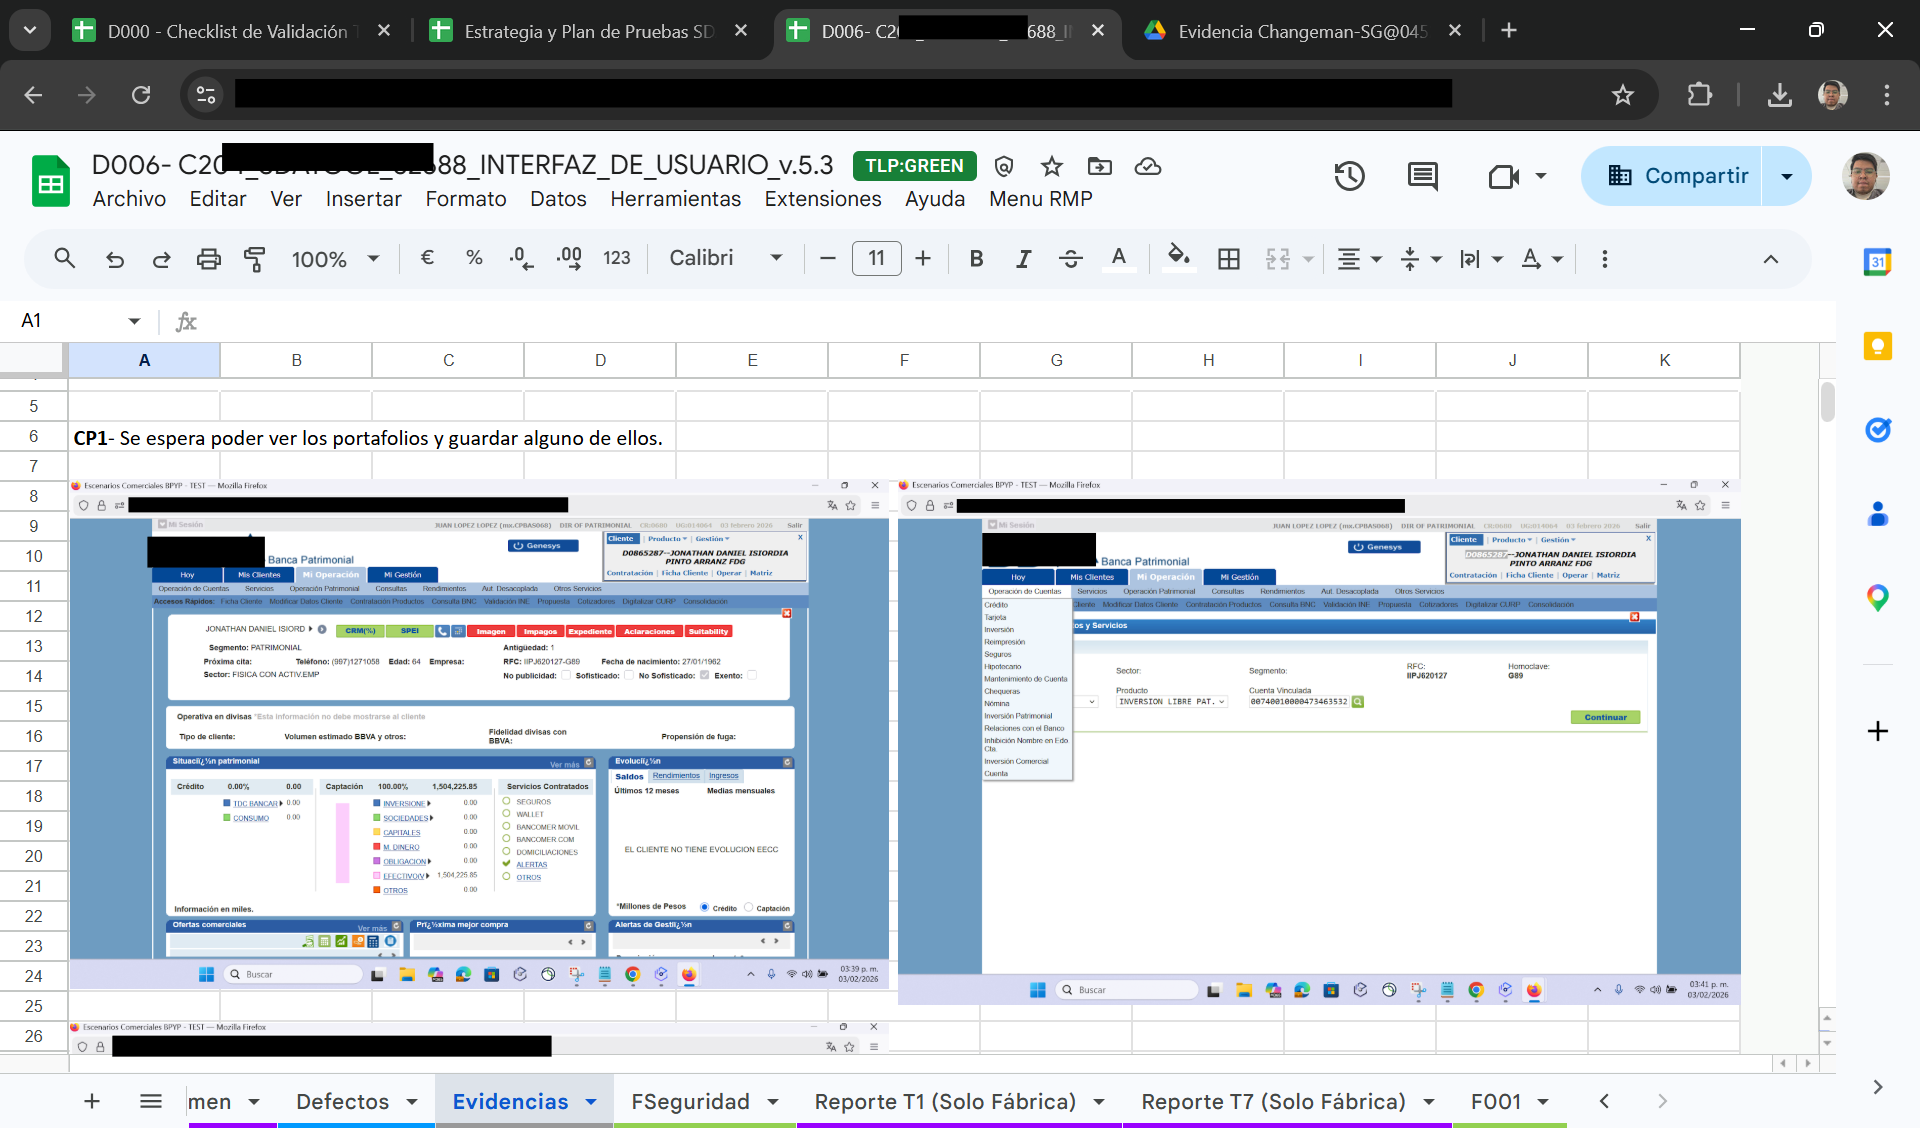
\includegraphics[width=0.95\textwidth]{E9/E5.png}
    \caption{Resultado de verificación técnica con confirmación de ejecución exitosa, sin errores identificados dentro del alcance evaluado.}
\end{figure}

\begin{figure}[H]
    \centering
    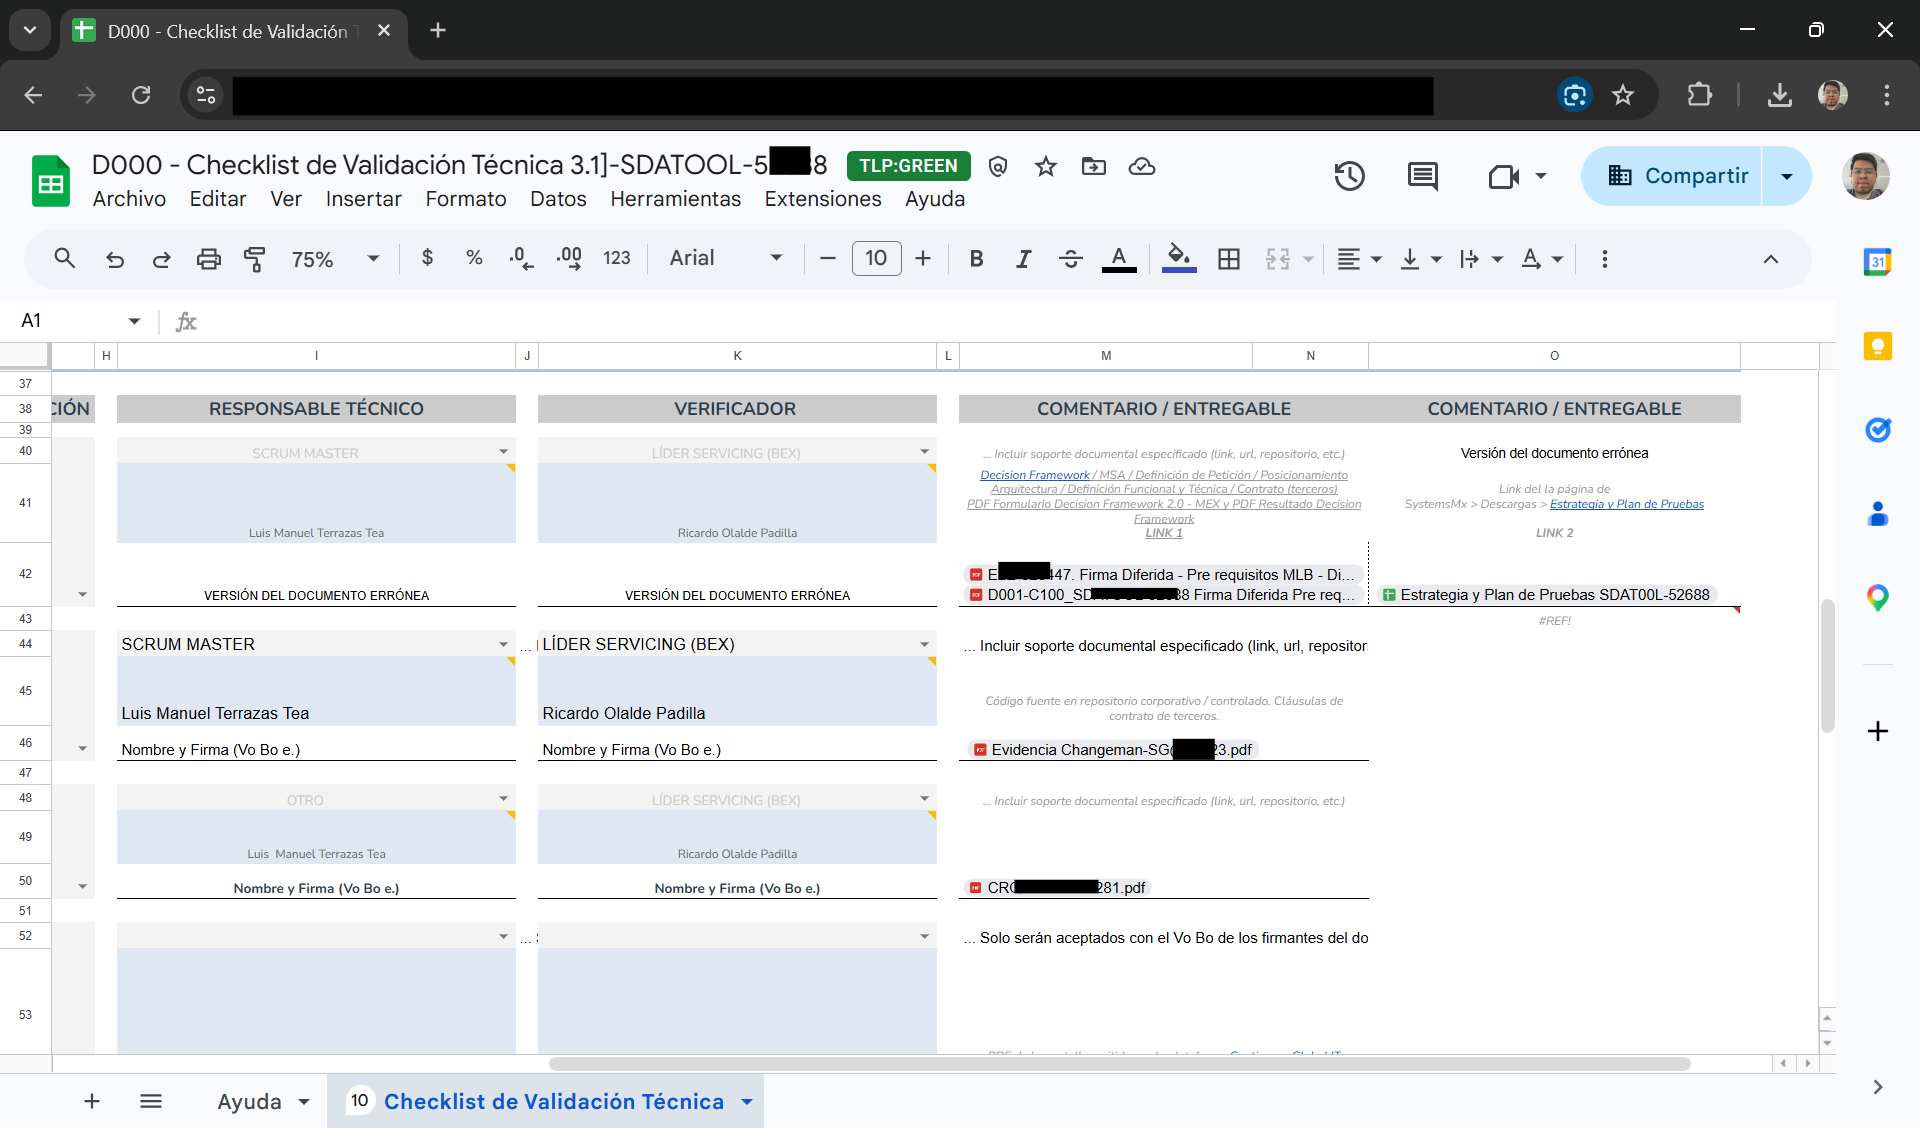
\includegraphics[width=0.95\textwidth]{E9/E6.png}
    \caption{Checklist de validación técnica con responsables, verificadores, observaciones y soportes documentales integrados como parte del proceso de aprobación técnica.}
\end{figure}

\end{document}
